\chapter{Motivation} 

In distributed systems and the involved technologies, a significant amount of
terms and definitions have been given in the literature. The first part of this
technology research aims to achieve more clarity in this confusing and oftentimes
ambiguous \textit{jungle of terminology}, where the focus lies on topics that
are related to Apache Kafka. After defining basic concepts for referencing
during this thesis, we go deeper into the technology and components of Apache
Kafka itself.

\begin{figure}
\centering
    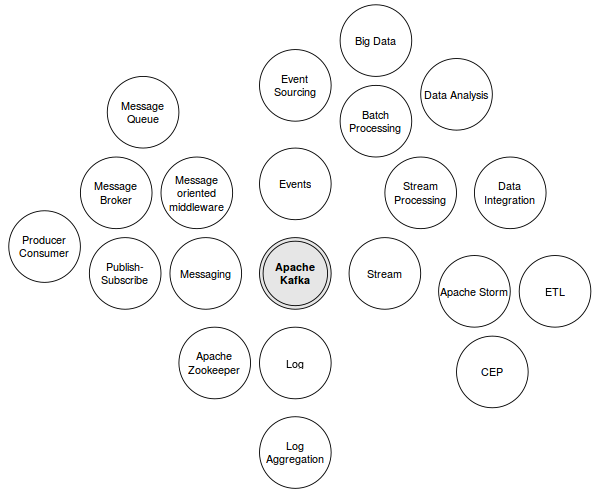
\includegraphics[width=0.6\textwidth]{images/jungle-of-terminology.png}
    \caption{\textit{Jungle of Terminology} related to Apache Kafka}
    \label{fig:jungle-of-terminology}
\end{figure}
